\chapter{Il modello SIEM}
\label{chap:Il modello SIEM}


%\section{Introduzione}
%\label{sec:Introduzione}

Oggi il cyber crimine è una vera e propria industria, con obiettivi ben definiti e “know how” per raggiungerli. \par
L’emergenza Covid-19 ha evidenziato questo fenomeno, mettendo in luce la necessità delle aziende a garantire la sicurezza delle proprie infrastrutture anche in ambienti non tradizionali, come nel caso dello smartworking.\par
Oltre alla consueta e ormai inevitabile crescita degli attacchi, nel corso del 2020 secondo Check Point Software (Cps), società israeliana specializzata nella sicurezza informatica, il numero totale di attacchi informatici segnalati a livello globale relativi al coronavirus è passato dai 200 pre-pandemia a oltre 5.000 al giorno (Petrucciani, 2020) :



\begin{figure}[h]
    \begin{center}
        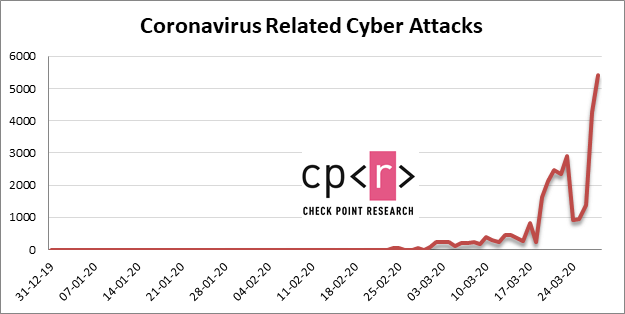
\includegraphics[scale=0.6]{images/1_modelloSIEM_img/cpr-coronavirus-graph-2-april.png}
    \end{center}
    \caption{Report Check Point Research degli cyber attack durante l'inizio della pandemia COVID-19}
    \label{fig:Dashboard QRadar}
\end{figure}

\newpage

Oltre al problema di sicurezza sanitaria si è aggiunto anche il problema della sicurezza informatica. Secondo i dati Cps, l’84\% degli attacchi hanno riguardato attività di phishing. L’impatto sanitario ed economico del coronavirus non ha scoraggiato i cybercriminali, anzi è esattamente il contrario, sfruttano la situazione utilizzando la paura del coronavirus come esca (Petrucciani, 2020). \par
A fronte di questi contesti, i sistemi di sicurezza tradizionali non sono più sufficienti, la nuova sfida che si propone consiste nel:


\begin{center}
    \textit{sapere COSA STA SUCCEDENDO e non COSA È GIÀ SUCCESSO}
\end{center}

Ogni CISO (chief information security officer) che si rispetti sa benissimo che raggiungere il “traguardo” della sicurezza informatica è pura utopia. Si può considerare sicuro solo un sistema isolato, quindi non soggetto a contatti esterni.\par 
Considerando il fatto che è inconcepibile, ai giorni d’oggi, pensare di isolare completamente un infrastruttura, quindi è necessario intraprendere un percoso, nel quale viene definita una strategia di difesa del perimetro IT in funzione dei cambiamenti del contesto aziendale e tecnologico.

Negli ultimi anni sono emerse nuove tecnologie e strumenti che fino a pochi anni fa erano inavvicinabili per le medie e piccole aziende, per via dei costi, dei tempi e della complessità di implementazione.
Stiamo parlando dei sistemi SIEM, di seguito le soluzioni offerte dei maggiori vendor, sia per il mondo commerciale che opensource:



\begin{itemize}
    \item{IBM Qradar}; 
    \item{Splunk};
    \item{Alienvault OSSIM}.
\end{itemize}

\section{Definzione del modello}
\label{sec:Definzione del modello}

SIEM è l’acronimo di “Security Information and Event Management”, il termine è stato coniato da Amrit Williams e Mark Nicolett nel 2005, quando entrambi lavoravano per Gartner.\par
I SIEM devono rispondere all’esigenza che è sorta nel corso degli anni di applicare in maniera sistematica un’analisi computazionale di dati o statistiche inerenti alla sicurezza informatica, quest’analisi deve avvenire in tempo reale in modo da rilevare in maniera tempestiva attacchi mirati e violazioni dei dati (“data breaches”), altra necessità che i SIEM devono soddisfare è quella di raccogliere, memorizzare, analizzare e rendere disponibile in forma di report i dati provenienti dai log per esigenze di incident response, di compliance in ambito regolatorio o per attività di analisi forense (Cristiani, 2020).

\newpage

Le tecnologie SIEM aggregano dunque i dati corrispondenti agli eventi prodotti da dispositivi di sicurezza.\par

Tecnicamente il SIEM e’ la combinazione di due funzioni di management indispensabili per la cybersicurezza: quella delle informazioni/Log management (SIM) e quella degli eventi (SEM).\newline

Il SEM è una soluzione software che, in tempo reale, provvede al monitoraggio e alla gestione degli eventi che accadono all'interno della rete e sui vari sistemi di sicurezza, fornendo una correlazione e aggregazione tra essi. L’interfaccia è una console centralizzata, preposta ad attività di monitoraggio, segnalazione e risposta automatica a determinati eventi (Networkdigital360, 2019).\newline

Il SIM (Security Information Management), è una soluzione che automatizza il processo di raccolta e gestione dei log (ma non in tempo reale). I dati vengono raccolti e spediti ad un server centralizzato tramite l’utilizzo di software agent installati sui vari dispositivi del sistema monitorato. La possibilità di usufruire di spazi di archiviazione a lungo termine unita all'analisi dei dati consente la generazione di report personalizzati (Networkdigital360, 2019).\newline

La principale fonte dati del SIEM sono i log, ma hanno anche la capacità di elaborare le informazioni sotto altre forme, come il Netflow .
In generale, il SIEM riceve dati “grezzi”, i quali tramite un processo di normalizzazione possono essere utilizzati per eseguire le operazioni di correlazione e di detection di anomalie.\par
Le regole di correlazione sono indispensabili per individuare attacchi complessi, correlando eventi di sicurezza permettendo agli operatori di avere una visione chiara su cosa sta succedendo.\par
Inoltre e’ possibile integrare le funzioni di incident management con workflow automatizzati, denominate SOAR (Security Orchestration Automation and Response), alleggerendo di gran lunga il lavoro degli amministratori di sistema, essendo in grado di reagire in modo automatico agli eventi.\par
I maggiori vendor SIEM, hanno compreso la potenzialità dell’ intelligenza artificiale e machine learning, tant'è che ormai l’integrazione con tale tecnologia è diventato uno standard, incrementando nuove funzionalità e ottimizzando velocità e precisione dei sistemi.



\section{SIEM Next-Gen}
\label{sec:SIEM Next-Gen}

I SIEM hanno fatto la loro comparsa sul mercato nel 1997, con lo scopo di limitare i falsi positivi generati dagli IDS (Intrusion Detection System). Le successive evoluzioni puntavano nel migliorare la gestione dei big data da elaborare, ma persisteva la complessità delle fasi implementative e soprattutto la limitata scalabilità e integrazione con altri strumenti di sicurezza.\par
L’offerta dei vendor, infatti, aveva sovrastimato la capacità dei responsabili della sicurezza di gestire il cambio di passo introdotto da una soluzione SIEM.\par
Oggi i sistemi di nuova generazione non solo sono diventati più agili, modulari e flessibili ma offrono il massimo valore, con dei costi di implementazione e operativi decisamente inferiori, per questo sono adottati da ogni tipo di organizzazione che ha a cuore la sicurezza, indipendentemente dalle dimensioni e dai settori di riferimento.\par

\begin{figure}[h]
    \begin{center}
        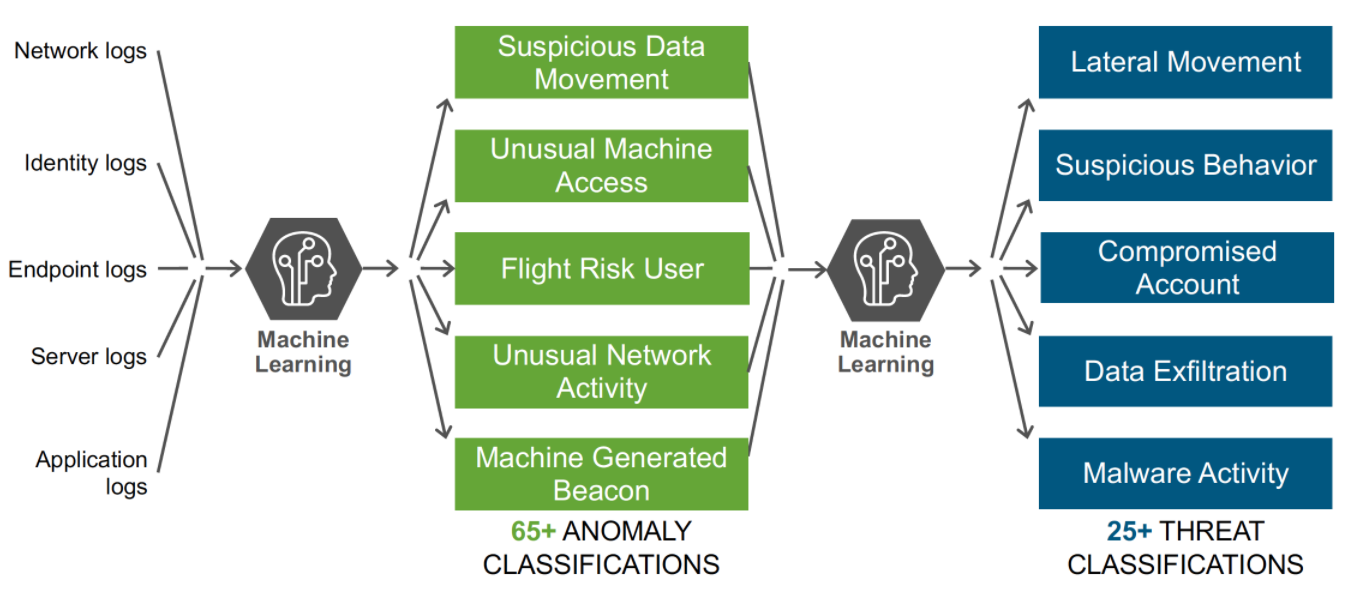
\includegraphics[width=0.95\columnwidth]{images/1_modelloSIEM_img/splunk_UBA.png}
    \end{center}
    \caption{Uso del machine learning nel SIEM Splunk}
    \label{fig:Uso del machine learning nel SIEM Splunk}
\end{figure} 


Il vero salto generazionale è stato segnato dall’integrazione con la tecnologia dell’Intelligenza Artificiale e, in particolare, il Machine Learning, ottenendo importanti vantaggi: 


\begin{itemize}
    \item\textbf{Affrontare i rischi sconosciuti:} Identificando gli attacchi zero-day e le minacce interne che appaiono molto simili alla normale attività dell'utente.; 
    \item\textbf{Identificare le anomalie nel comportamento dell'utente o del dispositivo:} Modellando il comportamento normale degli utenti, dei dispositivi di rete o di gruppi e identificando quando un utente o un dispositivo si discosta dalla norma e mostra un comportamento sospetto;
    \item\textbf{Identificare anomalie della network:} Modella il comportamento normale della rete e se identifica se qualcosa di strano sta accadendo rispetto a uno specifico segmento di rete, tipo di traffico, ora del giorno o periodo;
    \item\textbf{Dimiuire I falsi positivi:} Gli algoritmi di machine learning utilizzati nell'ambito dell'analisi comportamentale possono aiutare a controllare la percentuale di falsi positivi attraverso il monitoraggio e la regolazione delle policy attivate;
    \item\textbf{Incident response automatico: } L'esecuzione di playbook di sicurezza automatizzati in risposta alle minacce rilevate dalle tecniche di apprendimento automatico.
\end{itemize}

Per contro, l’AI può essere sfruttata anche da malintenzionati per mettere in atto attacchi sempre più sofisticati, come per esempio la creazione di nuovi malware in grado di sviluppare comportamenti adattativi o lo sviluppo automatico di campagne di phishing efficaci (Antonielli A. \& Dragoni G. , 2020).
